\documentclass[aspectratio=43]{beamer}

% Text packages to stop warnings
\usepackage{lmodern}
\usepackage{textcomp}
\usepackage{listings}

% Themes
\usetheme{Boadilla}
\setbeamertemplate{footline}[page number]{}
\setbeamertemplate{navigation symbols}{}

% Suppress the navigation bar
\beamertemplatenavigationsymbolsempty

\lstset{basicstyle=\scriptsize, frame=single}

\newenvironment{changemargin}[1]{% 
  \begin{list}{}{% 
    \setlength{\topsep}{0pt}% 
    \setlength{\leftmargin}{#1}% 
    \setlength{\rightmargin}{1em}
    \setlength{\listparindent}{\parindent}% 
    \setlength{\itemindent}{\parindent}% 
    \setlength{\parsep}{\parskip}% 
  }% 
  \item[]}{\end{list}} 

\title{Lecture 06---A1; Race Conditions;\\ More Synchronization; Async I/O}
\date{January 21, 2014}

\begin{document}

%%%%%%%%%%%%%%%%%%%%%%%%%%%%%%%%%%%%%%%%%%%%%%%%%%%%%%%%%%%%%%%%%%%%%%%%%%%%%%%%
\begin{frame}[plain]
  \titlepage
\end{frame}
%%%%%%%%%%%%%%%%%%%%%%%%%%%%%%%%%%%%%%%%%%%%%%%%%%%%%%%%%%%%%%%%%%%%%%%%%%%%%%%%

%%%%%%%%%%%%%%%%%%%%%%%%%%%%%%%%%%%%%%%%%%%%%%%%%%%%%%%%%%%%%%%%%%%%%%%%%%%%%%%%
\begin{frame}
  \frametitle{Roadmap}

  \Large
    \begin{changemargin}{2cm}
  Past: Modern Hardware, Threads \\[1em]

  Now: A1 discussion, non-blocking I/O;\\[1em]

  Next: Race Conditions, Locking
    \end{changemargin}
  
\end{frame}
%%%%%%%%%%%%%%%%%%%%%%%%%%%%%%%%%%%%%%%%%%%%%%%%%%%%%%%%%%%%%%%%%%%%%%%%%%%%%%%%

%%%%%%%%%%%%%%%%%%%%%%%%%%%%%%%%%%%%%%%%%%%%%%%%%%%%%%%%%%%%%%%%%%%%%%%%%%%%%%%%
\begin{frame}
  \frametitle{Last Time}

  \begin{changemargin}{2.5cm}
  \begin{itemize}
    \item Processes vs threads.
    \vfill
    \item Creating, joining and exiting POSIX threads.\\
       Remember, they are 1:1 with kernel threads and can run in parallel on
      multiple CPUs.
    \vfill
    \item Difference between \structure{joinable} and \structure{detached} threads.
    \vfill
  \end{itemize}
  \end{changemargin}
\end{frame}
%%%%%%%%%%%%%%%%%%%%%%%%%%%%%%%%%%%%%%%%%%%%%%%%%%%%%%%%%%%%%%%%%%%%%%%%%%%%%%%%

\part{Assignment 1}
\frame{\partpage}

%%%%%%%%%%%%%%%%%%%%%%%%%%%%%%%%%%%%%%%%%%%%%%%%%%%%%%%%%%%%%%%%%%%%%%%%%%%%%%%%

\begin{frame}
  \frametitle{Your Task}

  \hspace*{2em} Re-assemble the picture:

  \begin{center}
  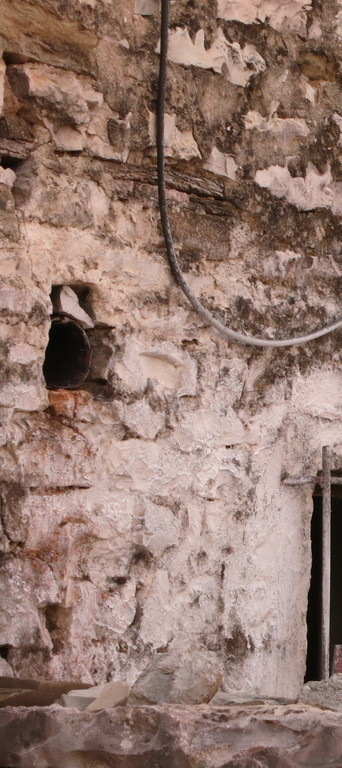
\includegraphics[width=.25\textwidth]{L06/part1} \qquad
  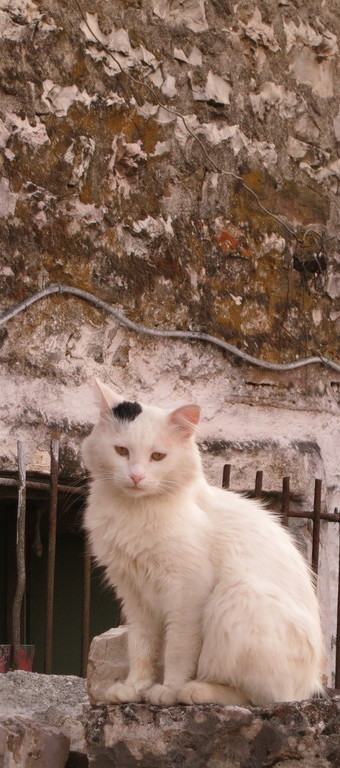
\includegraphics[width=.25\textwidth]{L06/part2} \qquad
  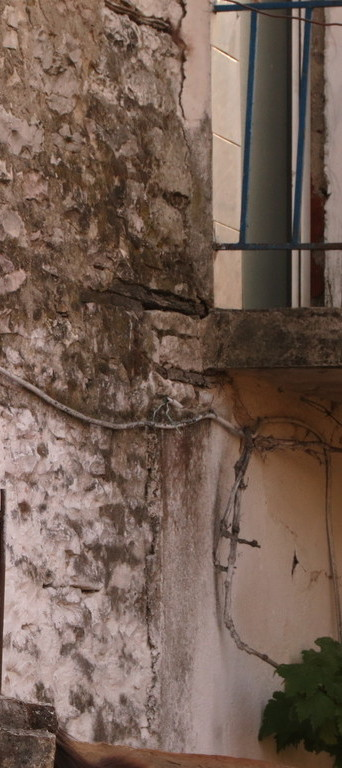
\includegraphics[width=.25\textwidth]{L06/part3}
  \end{center}
\end{frame}

%%%%%%%%%%%%%%%%%%%%%%%%%%%%%%%%%%%%%%%%%%%%%%%%%%%%%%%%%%%%%%%%%%%%%%%%%%%%%%%%

%%%%%%%%%%%%%%%%%%%%%%%%%%%%%%%%%%%%%%%%%%%%%%%%%%%%%%%%%%%%%%%%%%%%%%%%%%%%%%%%

\begin{frame}
  \frametitle{What I provide}

  \begin{changemargin}{2em}
    Serial C code:
\begin{itemize}
  \item uses curl to fetch the image over the network;
  \item uses libpng to stitch together the image.
\end{itemize}
    Plus, a web API to provide images to you.

  \end{changemargin}

\end{frame}

%%%%%%%%%%%%%%%%%%%%%%%%%%%%%%%%%%%%%%%%%%%%%%%%%%%%%%%%%%%%%%%%%%%%%%%%%%%%%%%%

%%%%%%%%%%%%%%%%%%%%%%%%%%%%%%%%%%%%%%%%%%%%%%%%%%%%%%%%%%%%%%%%%%%%%%%%%%%%%%%%
\begin{frame}
  \frametitle{What you hand in}

  \begin{changemargin}{2em}
    Part 1: pthreads parallelized implementation.\\
\begin{itemize}
  \item really easy!
  \item (also, analyze your speedups in the report.)
\end{itemize}

    Part 2: nonblocking I/O implementation.\\
\begin{itemize}
  \item more challenging;
  \item lecture today will help.
\end{itemize}

Also Parts 0, 3: analysis \& discussion.

  \end{changemargin}

\end{frame}

%%%%%%%%%%%%%%%%%%%%%%%%%%%%%%%%%%%%%%%%%%%%%%%%%%%%%%%%%%%%%%%%%%%%%%%%%%%%%%%%

%%%%%%%%%%%%%%%%%%%%%%%%%%%%%%%%%%%%%%%%%%%%%%%%%%%%%%%%%%%%%%%%%%%%%%%%%%%%%%%%
\begin{frame}
  \frametitle{Tour of the code}

  \begin{changemargin}{2em}
    main loop: while still missing some fragments,
    \begin{itemize}
      \item retrieve a fragment over the network;
      \item copy bits into our array;
    \end{itemize}
    Then, write all the bits in one PNG file.
  \end{changemargin}

\end{frame}
%%%%%%%%%%%%%%%%%%%%%%%%%%%%%%%%%%%%%%%%%%%%%%%%%%%%%%%%%%%%%%%%%%%%%%%%%%%%%%%%

%%%%%%%%%%%%%%%%%%%%%%%%%%%%%%%%%%%%%%%%%%%%%%%%%%%%%%%%%%%%%%%%%%%%%%%%%%%%%%%%
\begin{frame}[fragile]
  \frametitle{Notable bits I: retrieving the file}

  \begin{changemargin}{2em}

    Here's how I retrieve the file:

    \begin{lstlisting}
  curl_easy_setopt(curl, CURLOPT_URL, url);

  // do curl request; check for errors
  res = curl_easy_perform(curl);
    \end{lstlisting}

    But wait! I had to tell curl where to put the file:

    \begin{lstlisting}
  struct bufdata bd; 
  bd.buf = input_buffer; 
  curl_easy_setopt(curl, CURLOPT_WRITEFUNCTION, write_cb);
  curl_easy_setopt(curl, CURLOPT_WRITEDATA, &bd);
    \end{lstlisting}

    My {\tt write\_cb} callback function puts data in {\tt input\_buffer} (straightforward {\tt memcpy}-based
    implementation).

  \end{changemargin}
\end{frame}

%%%%%%%%%%%%%%%%%%%%%%%%%%%%%%%%%%%%%%%%%%%%%%%%%%%%%%%%%%%%%%%%%%%%%%%%%%%%%%%%
\begin{frame}
  \frametitle{Notable bits II: parsing the fragments}

  \begin{changemargin}{2em}

    Bunch of {\tt libpng} magic:\\

    \hspace*{1em} {\tt libpng} wants to put the image data in a {\tt png\_bytep *} array,
    where each element points to a row of pixels.\\[1em]

    My {\tt read\_png\_file} function allocates the data; caller must free.\\[1em]

    Then, {\tt paint\_destination} fills in the output array, \\pasting together
    the fragments.
  \end{changemargin}
\end{frame}
%%%%%%%%%%%%%%%%%%%%%%%%%%%%%%%%%%%%%%%%%%%%%%%%%%%%%%%%%%%%%%%%%%%%%%%%%%%%%%%%

%%%%%%%%%%%%%%%%%%%%%%%%%%%%%%%%%%%%%%%%%%%%%%%%%%%%%%%%%%%%%%%%%%%%%%%%%%%%%%%%
\begin{frame}
  \frametitle{Notable bits III: writing the output}
  \begin{changemargin}{2em}

    Well, not that notable. Symmetric to read.\\

    Note: be sure to free everything! (We'll check.)
  \end{changemargin}
\end{frame}
%%%%%%%%%%%%%%%%%%%%%%%%%%%%%%%%%%%%%%%%%%%%%%%%%%%%%%%%%%%%%%%%%%%%%%%%%%%%%%%%

%%%%%%%%%%%%%%%%%%%%%%%%%%%%%%%%%%%%%%%%%%%%%%%%%%%%%%%%%%%%%%%%%%%%%%%%%%%%%%%%
\begin{frame}
  \frametitle{Part (a): using pthreads}
  \begin{changemargin}{2em}
    You might need to refactor the code to parallelize it well.\\[1em]

    Start some threads. \\[1em] Justify why the threads are not interfering. Time the result.
  \end{changemargin}
\end{frame}

%%%%%%%%%%%%%%%%%%%%%%%%%%%%%%%%%%%%%%%%%%%%%%%%%%%%%%%%%%%%%%%%%%%%%%%%%%%%%%%%

%%%%%%%%%%%%%%%%%%%%%%%%%%%%%%%%%%%%%%%%%%%%%%%%%%%%%%%%%%%%%%%%%%%%%%%%%%%%%%%%
\begin{frame}
  \frametitle{Part (b): nonblocking I/O}
  \begin{changemargin}{2em}
    Main subject of this lecture. \\

    Will be more complicated than using threads!
  \end{changemargin}
\end{frame}

%%%%%%%%%%%%%%%%%%%%%%%%%%%%%%%%%%%%%%%%%%%%%%%%%%%%%%%%%%%%%%%%%%%%%%%%%%%%%%%%

%%%%%%%%%%%%%%%%%%%%%%%%%%%%%%%%%%%%%%%%%%%%%%%%%%%%%%%%%%%%%%%%%%%%%%%%%%%%%%%%
\begin{frame}
  \frametitle{Part (b)': JavaScript}
  \begin{changemargin}{2em}
    As an alternate option, you may use either {\tt node.js} or\\ client-side
    JavaScript to do the nonblocking I/O.\\[1em]

    Let me know if you want to do this. You are on your own, though.
  \end{changemargin}
\end{frame}
%%%%%%%%%%%%%%%%%%%%%%%%%%%%%%%%%%%%%%%%%%%%%%%%%%%%%%%%%%%%%%%%%%%%%%%%%%%%%%%%

%%%%%%%%%%%%%%%%%%%%%%%%%%%%%%%%%%%%%%%%%%%%%%%%%%%%%%%%%%%%%%%%%%%%%%%%%%%%%%%%
\part{Asynchronous/non-blocking I/O}
\frame{\partpage}
%%%%%%%%%%%%%%%%%%%%%%%%%%%%%%%%%%%%%%%%%%%%%%%%%%%%%%%%%%%%%%%%%%%%%%%%%%%%%%%%

%%%%%%%%%%%%%%%%%%%%%%%%%%%%%%%%%%%%%%%%%%%%%%%%%%%%%%%%%%%%%%%%%%%%%%%%%%%%%%%%
\begin{frame}
  \frametitle{Juicy Quotes}
  \begin{changemargin}{2em}

  \fbox{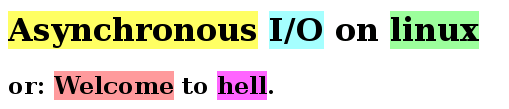
\includegraphics[width=.7\textwidth]{L06/aio-linux.png}}\\
{\scriptsize (mirrored at \url{compgeom.com/~piyush/teach/4531_06/project/hell.html})}
   \\[3em]

   ``Asynchronous I/O, for example, is often infuriating.''\\
--- Robert Love. {\em Linux System Programming, 2nd ed, } page 215.
  
  \end{changemargin}
\end{frame}
%%%%%%%%%%%%%%%%%%%%%%%%%%%%%%%%%%%%%%%%%%%%%%%%%%%%%%%%%%%%%%%%%%%%%%%%%%%%%%%%

%%%%%%%%%%%%%%%%%%%%%%%%%%%%%%%%%%%%%%%%%%%%%%%%%%%%%%%%%%%%%%%%%%%%%%%%%%%%%%%%
\begin{frame}[fragile]
  \frametitle{Why non-blocking I/O?}
  \begin{changemargin}{2em}
  Consider some I/O:

\begin{changemargin}{3em}
\begin{minipage}{.5\textwidth}
\begin{lstlisting}
    fd = open(...);
    read(...);
    close(fd);
  \end{lstlisting}
\end{minipage}
\end{changemargin}

  Not very performant---under what conditions do we lose out?
  \end{changemargin}
\end{frame}
%%%%%%%%%%%%%%%%%%%%%%%%%%%%%%%%%%%%%%%%%%%%%%%%%%%%%%%%%%%%%%%%%%%%%%%%%%%%%%%%

%%%%%%%%%%%%%%%%%%%%%%%%%%%%%%%%%%%%%%%%%%%%%%%%%%%%%%%%%%%%%%%%%%%%%%%%%%%%%%%%
\begin{frame}[fragile]
  \frametitle{Mitigating I/O impact}
  \begin{changemargin}{2em}
    So far: can use threads to mitigate latency.\\

    What are the disadvantages?
    \only<2>{
      \begin{itemize}
        \item race conditions
        \item overhead/max \# of thread limitations
      \end{itemize}
    }
  \end{changemargin}
\end{frame}
%%%%%%%%%%%%%%%%%%%%%%%%%%%%%%%%%%%%%%%%%%%%%%%%%%%%%%%%%%%%%%%%%%%%%%%%%%%%%%%%

%%%%%%%%%%%%%%%%%%%%%%%%%%%%%%%%%%%%%%%%%%%%%%%%%%%%%%%%%%%%%%%%%%%%%%%%%%%%%%%%
\begin{frame}[fragile]
  \frametitle{Live coding: forkbomb Patrick's laptop!}

\begin{center}
(well, threadbomb anyway)
\end{center}

\end{frame}
%%%%%%%%%%%%%%%%%%%%%%%%%%%%%%%%%%%%%%%%%%%%%%%%%%%%%%%%%%%%%%%%%%%%%%%%%%%%%%%%

%%%%%%%%%%%%%%%%%%%%%%%%%%%%%%%%%%%%%%%%%%%%%%%%%%%%%%%%%%%%%%%%%%%%%%%%%%%%%%%%
\begin{frame}[fragile]
  \frametitle{An Alternative to Threads}
  \begin{changemargin}{2em}
    Asynchronous/nonblocking I/O.\\[2em]

\begin{changemargin}{3em}
\begin{minipage}{.6\textwidth}
\begin{lstlisting}
    fd = open(..., O_NONBLOCK);
    read(...); // returns instantly!
    close(fd);
  \end{lstlisting}
\end{minipage}
\end{changemargin}

\begin{center}
~\\[1em]
$\cdots$\\[2em]


\includegraphics[width=.25\textwidth]{L06/Easy_button.JPG}
\end{center}
\hfill {\scriptsize (credit: Yskyflyer, Wikimedia Commons)}

  \end{changemargin}
\end{frame}
%%%%%%%%%%%%%%%%%%%%%%%%%%%%%%%%%%%%%%%%%%%%%%%%%%%%%%%%%%%%%%%%%%%%%%%%%%%%%%%%

%%%%%%%%%%%%%%%%%%%%%%%%%%%%%%%%%%%%%%%%%%%%%%%%%%%%%%%%%%%%%%%%%%%%%%%%%%%%%%%%
\begin{frame}
  \frametitle{Not Quite So Easy: Live Demo}
  \begin{changemargin}{2em}
    Doesn't work on files---they're always ready. Only e.g. sockets.
  \end{changemargin}
\end{frame}
%%%%%%%%%%%%%%%%%%%%%%%%%%%%%%%%%%%%%%%%%%%%%%%%%%%%%%%%%%%%%%%%%%%%%%%%%%%%%%%%

%%%%%%%%%%%%%%%%%%%%%%%%%%%%%%%%%%%%%%%%%%%%%%%%%%%%%%%%%%%%%%%%%%%%%%%%%%%%%%%%
\begin{frame}
  \frametitle{Other Outstanding Problem with Nonblocking I/O}
  \begin{changemargin}{2em}
    How do you know when I/O is ready to be queried?

    \only<2>{\begin{itemize} 
      \item polling ({\tt select}, {\tt poll}, {\tt epoll})
      \item interrupts (signals)
      \end{itemize}
    }
  \end{changemargin}
\end{frame}
%%%%%%%%%%%%%%%%%%%%%%%%%%%%%%%%%%%%%%%%%%%%%%%%%%%%%%%%%%%%%%%%%%%%%%%%%%%%%%%%

\end{document}
